\section{유효 온도 (effective temperature)}

\pagestyle{headings}
\markboth{유효 온도 (effective temperature)\hfill Kiehyun Park\hfill}

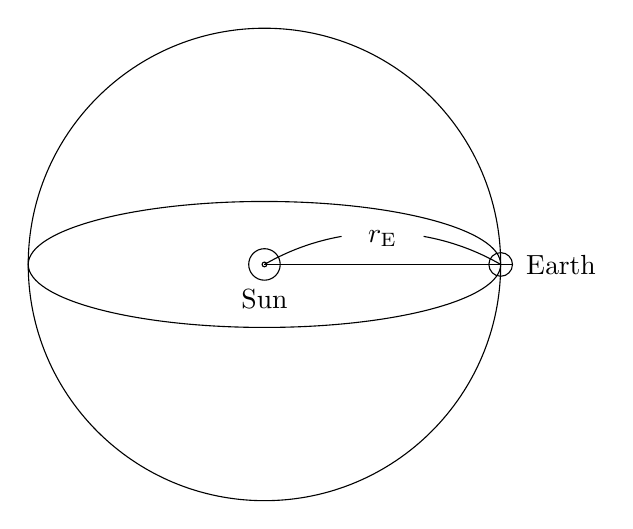
\begin{tikzpicture}[scale = 1, xshift = 1cm]
	\draw (5,2) circle (3cm);
	\draw (5,2) ellipse (3cm and 0.8cm);
	\draw (5,2) circle (0.03cm);
	\draw (5,2) circle (0.2cm) node[below, yshift=-0.2cm] {Sun};
	\draw (8,2) circle (0.15cm) node[right, xshift=0.2cm] {Earth};
	\draw (5,2) -- (8,2) node[above, xshift=-1.5cm, yshift=0.1cm] {$r_{\mathrm{E}}$};
	\draw (5,2) arc (120:100:3cm);
	\draw (8,2) arc (60:80:3cm);
	\draw (7.85,2) -- (8.15,2);
	\draw (8,1.85) -- (8,2.15);
\end{tikzpicture}

\vspace{1cm}
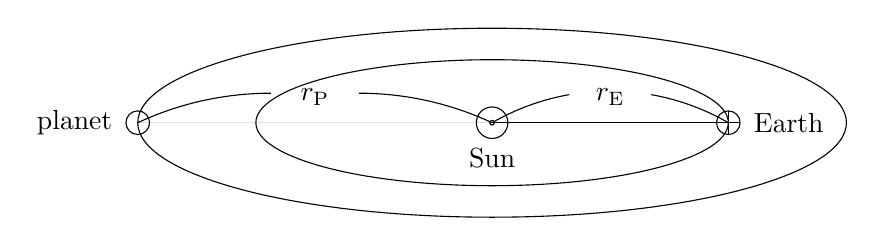
\begin{tikzpicture}[scale = 1, xshift = 1cm]
	\draw (5,2) ellipse (3cm and 0.8cm);
	\draw (5,2) ellipse (4.5cm and 1.2cm);
	\draw (5,2) circle (0.03cm);
	\draw (5,2) circle (0.2cm) node[below, yshift=-0.2cm] {Sun};
	\draw (8,2) circle (0.15cm) node[right, xshift=0.2cm] {Earth};
	\draw (5,2) -- (8,2) node[above, xshift=-1.5cm, yshift=0.1cm] {$r_{\mathrm{E}}$};
	\draw (5,2) arc (120:100:3cm);
	\draw (8,2) arc (60:80:3cm);
	\draw (0.5,2) circle (0.15cm) node[left, xshift=-0.2cm] {planet};
	\fill (5,2) -- (0.5,2) node[above, xshift=2.25cm, yshift=0.1cm] {$r_{\mathrm{P}}$};
	\draw (0.5,2) arc (115:90:4cm);
	\draw (5,2) arc (65:90:4cm);
	\draw (7.85,2) -- (8.15,2);
	\draw (8,1.85) -- (8,2.15);
\end{tikzpicture} 
	
\vspace{1cm}
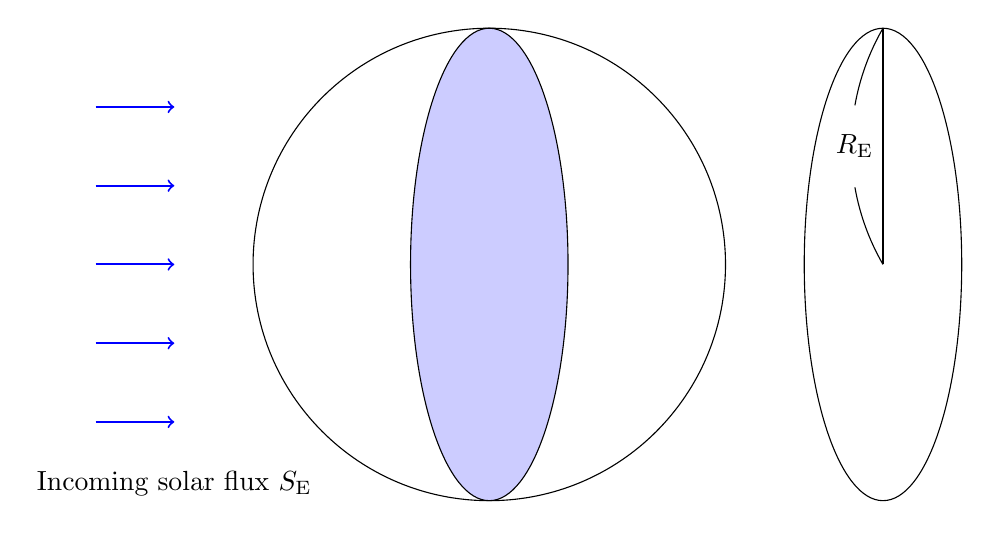
\begin{tikzpicture}[scale = 1, xshift = 1cm]
	\draw [line width=0.25mm, blue] [->] (0,0) -- (1,0) node[black, below, yshift=-0.5cm] {Incoming solar flux $S_{\mathrm{E}}$};
	\draw [line width=0.25mm, blue] [->] (0,1) -- (1,1);
	\draw [line width=0.25mm, blue] [->] (0,2) -- (1,2);
	\draw [line width=0.25mm, blue] [->] (0,3) -- (1,3);
	\draw [line width=0.25mm, blue] [->] (0,4) -- (1,4) ;
	
	\draw (5,2) circle (3cm);
	
	\fill [blue!20!white] (5,2) ellipse (1cm and 3cm) ;
	\draw (5,2) ellipse (1cm and 3cm) ;
	\draw (10,2) ellipse (1cm and 3cm);
	\draw (10,2) -- (10,5) node[left, yshift=-1.5cm] {$R_{\mathrm{E}}$};
	\draw (10,2) arc (210:190:3cm);
	\draw (10,5) arc (150:170:3cm);
\end{tikzpicture}


\begin{figure*}[h]
	\begin{tikzpicture}[rounded corners=3mm]
	\path node[rectangle,draw=green,fill=green!8,inner sep=.70cm] 
	{\parbox[t][15.5cm]{\textwidth-1.4cm-\fboxrule}
		{\question 
			* 행성의 유효 온도를 구하시오.
			\begin{solutionorlines}[15cm]

			* 지구에서의 태양 상수는
			$S_{\mathrm{E}} = \dfrac{L_{\odot}}{4\pi r_{\mathrm{E}}^{2}}$

			* 행성의 태양 상수($ S_{\mathrm{P}}$)와 지구의 태양 상수 $S_{\mathrm{E}}$는 
			$ S_{\mathrm{P}} = S_{\mathrm{E}}\left(\dfrac{r_{\mathrm{E}}}{r_{\mathrm{P}}}\right)^{2}$
			
			* 지구가 받는 태양 복사 에너지는  
			$\pi R_{\mathrm{E}}^{2} S_{\mathrm{E}}$

			* 행성이 받는 태양 복사 에너지는 
			$ \pi R_{\mathrm{P}}^{2} S_{\mathrm{E}}\left(\dfrac{r_{\mathrm{E}}}{r_{\mathrm{P}}}\right)^{2}$
			
			* 알베도($A$)를 고려하면 
			$ I_{\mathrm{P}}^{\downarrow} = (1-A)\pi R_{\mathrm{P}}^{2} S_{\mathrm{E}}\left(\dfrac{r_{\mathrm{E}}}{r_{\mathrm{P}}}\right)^{2}$
			
			* Stefan-Boltzmann 법칙에 따라 행성이 방출하는 복사 에너지량은
			$ I_{\mathrm{P}}^{\uparrow} = 4\pi R_{\mathrm{P}}^{2} \sigma T^{4}$
			
			* 따라서 행성의 유효 온도는
			$ T_{e} = \sqrt[4]{\dfrac{(1-A) S_{\mathrm{E}}}{4 \sigma}} \sqrt{\dfrac{r_{\mathrm{E}}}{r_{\mathrm{P}}}} $
			
			유효 온도는 행성과 태양과의 거리, 알베도에 의해 결정되며 대기의 구성 성분이나 밀도 등의 물리적 성질과는 무관하다.
			
			그러나 실제로 대기를 투과한 태양광이 대기의 구성 성분이나 지면에 흡수되고, 또 재방출 되는 복잡한 과정을 통하여 온도가 결정되므로 이러한 온도를 복사 온도(radiative temperature)라 한다. 
			실제 표면 온도는 행성의 유효온도에 대기의 온실효과 등이 더해져서 결정되어진 온도이다. 
			\end{solutionorlines}
	}};
	\end{tikzpicture}
\end{figure*}


\end{questions}
%(https://solarsystem.nasa.gov/system/resources/detail_files/681_ptemp.jpg)